\documentclass[16pt,answers]{exam}
\author{Nima Poshtiban}
\title{Assignments of Arithmetic}
\usepackage{datetime}
\usepackage{amsmath}
\usepackage[utf8]{inputenc}
\usepackage{hyperref}
\usepackage{color}
\usepackage{graphics}
\newdate{date}{{26}{10}{2025}}
\date{\displaydate{date}}
\usepackage{float}

\begin{document}
	\maketitle
	\tableofcontents
	\pagebreak
	\section{Assignment No.1}
\paragraph{}
\textbf{Unconventional radices}
\begin{questions}
\question Convert the negabinary number $\mathbf{(0001 1111 0010 1101)_{-two}}$ to radix 16
	(hexadecimal).\label{a}
	\begin{solution}[space]
		From the Radix we can elicit the base logic for solving this problem\newline
		\begin{enumerate}
			\item Assuming the initial index is 1, Odd digits represents positive values whereas even digits are the quite opposite.
			\item Applying the deduction, a mathematical formula has been extracted from the logic:
			\[
			  0001 1111 0010 1101 \Longrightarrow \sum_{i=1}^{16}{(d_{i})\times2^{i-1}\times(-1)^{i} }
			\]
			\item Calculating the initial value:
			\(-2^{0} + -2^{2} + -2^{3} + -2^{5}  + - 2^{8}  + -2^{9} + -2^{10} + -2^{11} + -2^{12} \Longrightarrow 2781_{decimal}\)
			\item Conversion from \(radix=10\) to \(radix=16\)
			doing the chain division and residue operations the result is \( ADD_{radix=16} \)
		\end{enumerate}
	\end{solution}
\question Repeat part \ref{a} for radix $\mathbf{-16}$ (negahexadecimal).
	\begin{solution}[space]
	using the general conversion formula
	\[N=\sum_{i=0}^{n}{a_{i}(radix)^{i}}\]
	Step 1. from the privious solotion the \textbf{radix=10} value is \textbf{2781}, Applying the conversion
	\[
		\Longrightarrow \frac{2781}{-16} \Rightarrow q=-173\,,r=-3+16 = D
	\]
	Step 2. continue until quotient=0
	\[
		\Longrightarrow \frac{-173}{-16} \Rightarrow q=11\,r=-13+16 = 3  
	\]
	\[
		\Longrightarrow \frac{11}{-16} \Rightarrow q=0\,,r= -5 + 16 = B
	\]
	Step 3. put the numbers back together by LSF convention
	\[
		\Rightarrow B3D_{-16}
	\]
\end{solution}
\question Derive a procedure for converting numbers from radix r to radix -r and vice
versa.
\begin{solution}
	in negative radices unlike positive radices odd digits are considered as negative numbers. thereby negative radices can be thought as  additions and subtractions of powers. hence\[
		Nbit(radix)=Mbit(-radix),\quad where\,\, M = N+1
	\]
	\[
		\Rightarrow N_{-r}\,=   \sum_{i=0}^{n}{odd\,digits} - \sum_{i=0}^{n}{even\,digits}
	\]
	\[
		\Rightarrow  N_{+r}\,= \sum_{i=0}^{n}{even\,digits} +  \sum_{i=0}^{n}{odd\,digits}
	\]
	The notice able point is if radix is positive we have two summation with positive sign between whereas for negative radix, the summations juxtapose with each other and the sign will change into negative
\end{solution}
\question An h-bit comparator is a circuit with two \textbf{h-bit} \textbf{unsigned binary} inputs, x and y,
and two binary outputs designating the conditions \(x < y\) and \(x > y\). Sometimes a
third output corresponding to x = y is also provided, but we do not need it for this
problem.
\begin{enumerate}
	\item Present the design of a 4-bit comparator.
	\begin{solution}
		I'll start with using binary encoding. since the third-state does not matter we need two outputs, just like the normal comparator but with only to output (s1,s0), this if s1 is set (10) y is larger otherwise s0 is set (01) which means x is larger  \\
		\begin{figure}[H]
			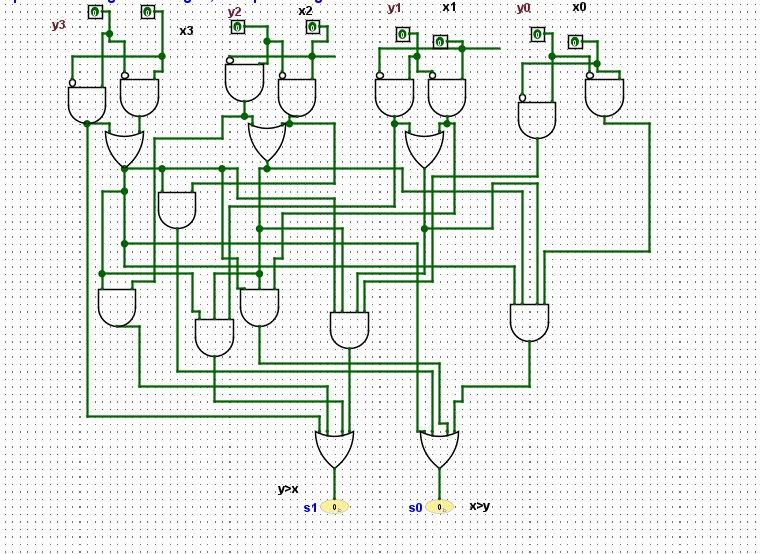
\includegraphics{4bc.jpg}
		\end{figure}
	\end{solution}
	\item Show how five 4-bit comparator can be cascaded to compare two 16-bit
	numbers.
	\begin{solution}
		using the previous comparator logic, we use each 4-bit comparator in parallel with each other, finally we add two OR gates just like before but this time each OR gate has 4 inputs from the left 4OR gate of each 4-comparator and doing OR just like before, same goes for the right 4ORs. the result is either 10 or 01, just like before 
	\end{solution}
	\item Show how a three-level tree of 4-bit comparators can be used to compare two
	28-bit numbers. Try to use as few 4-bit comparator blocks as possible.
	\item Generalize the result of part b to derive a synthesis method for large
	comparators built from a cascaded chain of smaller comparators.
\end{enumerate}

\question Left/right shifting is used to double/halve the magnitude of unsigned binary
integers.
\begin{enumerate}
	\item How can we use shifting to accomplish the same for 1’s- or 2’s-complement
	numbers?
	\begin{solution}
		Consider the (8bit)number \(10_{decimal}\) using arithmetic shift left will double it's amount
		\[
			00001010_{2} \Rightarrow 000101000_{2}
		\]
		Now Comparing the 1's-complement of \(10_{decimal}\) before and after arithmetic shift left we have:
		\[
			11110101_{2} \Longrightarrow 11101111_{2}
		\]
		
		Albeit using arithmetic shift left, 1's-complement has used circular shift left. The same thing stands for arithmetic shift right.\\
		Conclusion: \textbf{1's-Complement} need to do\textbf{ Circular Shift} instead of \textbf{Arithmetic Shift} operations.\\
			\textbf{2's Complement}\\
		For 2's-complement based on the definition, the following example shows that for every arithmetic shift left operations by a number, there\textbf{ will be two} arithmetic shift left for the 2's-complement number:\[
			0000 1010_{2} \Rightarrow 0010 1000_{2}
		\]
		before and after arithmetic shift left we have:
		\[
			1111 0110_{2} \Rightarrow 1101 1000_{2}
		\]
	
		For arithmetic shift right we have \[
			 0000 1010_{2} \Rightarrow0000 0101_{2}
		\]
		before and after arithmetic shift right we have:
		\[
			1111 0110_{2} \Rightarrow 1111 1011_{2}
		\]
		Thus for each Arithmetic Right Shift, we have a \textbf{circular left shift}\\
		Conclusion: \textbf{2's-Complement follows the same rule for  Shift Left  but for  Shift Right it will do a Circular Shift Left ! }
	\end{solution}
	
	\item What is the procedure for doubling or halving a biased number?
	\begin{solution}
		For making this possible, first eliminate the bias value then do the Shifts and then add the Bias value back
	\end{solution}
\end{enumerate}
	\question Discuss the effect of the end-around carry needed for 1’s-complement addition on
	the worst-case carry propagation delay and the total addition time.
	\begin{solution}
		There will be two extra addition which means 2 extra delays
	\end{solution}
	
	\question Discuss the 10’s- and 9’s-complement number systems that are the radix-10 counterparts to 2’s- and 1’s-complement representations. In particular, describe any
	changes that might be needed in arithmetic algorithms.
	
	\question
	Show the subtraction of 2’s-complement numbers in extended dot notation

\end{questions}



\end{document}